\documentclass{QD_2026}

\makeatletter
\setlength{\@fptop}{0pt}
\makeatother

% Additional packages not already provided by QD_2026.cls
\usepackage{graphicx}
\usepackage{microtype}
\usepackage{amsfonts}

\sisetup{detect-all}
\graphicspath{{figures/}}

% Math macros used throughout the paper
\newcommand{\rps}{\mathrm{RPS}}
\newcommand{\revps}{\mathrm{rev}/\mathrm{s}}
\newcommand{\rsq}{R^{2}}

%%%%%%%%%%%%%%%%%%%%%%%%%%%%%%%%%%%%
% BEGIN DOCUMENT
%%%%%%%%%%%%%%%%%%%%%%%%%%%%%%%%%%%%
\begin{document}

%% Header image on 1st page -- do not modify
\begin{figure}[t!]
  \centering
  \includegraphics[keepaspectratio, width=0.6\textwidth]{QD2026_logo_cropped.pdf}
\end{figure}
\hfill
\hfill
%%

\selectlanguage{english}

%%%%%%%%%%%%%%%%%%%%%%%%%%%%%%%%%%%%
% FRONT MATTER
%%%%%%%%%%%%%%%%%%%%%%%%%%%%%%%%%%%%

\title{Rotor Speed Estimation from Drone Sound}
\QDsession{UAV Noise: Monitoring and Characterisation}  % TODO: update with actual session name

\author{
\bf{Author One}, Institution, Country, \email{author.one@institution.edu}
\and
\bf{Author Two}, Institution, Country, \email{author.two@institution.edu}
}

\maketitle

\author{}

\begin{abstract}
\textbf{Abstract}
The acoustic signature of a multirotor unmanned aerial vehicle~(UAV) is dominated
by rotor harmonics whose fundamentals are set by the instantaneous rotational
speeds~(RPS) of each rotor.
Recovering per-rotor RPS directly from a single-channel audio recording would
enable passive acoustic monitoring of drone state---flight-mode and manoeuvre
inference, payload and fault diagnostics, model-based source separation, and
conditioning signals for downstream speech or event-detection systems---without
access to onboard telemetry.
We present a first study of audio-only RPS estimation in the practically relevant
regime where the rotor signal is mixed with strong non-rotor sound.
We train a lightweight convolutional regressor that takes the log-magnitude
short-time Fourier transform of the mixture as input and outputs, at every STFT
frame, the four per-rotor speeds; the network is trained by frame-wise regression
against telemetry-aligned ground truth.
On synthetic mixtures of LibriSpeech utterances and real quadcopter recordings
from the DREGON dataset spanning $-30$ to $0$~dB signal-to-noise ratio, the model
attains a coefficient of determination $\rsq = 0.95$, a mean absolute error of
$0.56~\revps$, and a mean squared error of $5.15~(\revps)^{2}$ on held-out
mixtures.
The model remains accurate on out-of-distribution high-SNR free-flight recordings,
where the mean squared error stays close to its in-distribution value (factor of
$\approx 1.2$ against a level-matched in-distribution baseline), while two larger
complex-valued encoders trained on the same data degrade by factors of three to
five over the same shift.\\\\
\textbf{Keywords}: drone acoustics; rotor speed estimation; passive acoustic monitoring; harmonic noise; multirotor UAV
\end{abstract}

%%%%%%%%%%%%%%%%%%%%%%%%%%%%%%%%%%%%
% END OF FRONT MATTER
%%%%%%%%%%%%%%%%%%%%%%%%%%%%%%%%%%%%


%%%%%%%%%%%%%%%%%%%%%%%%%%%%%%%%%%%%
% DOCUMENT MAIN SECTIONS
%%%%%%%%%%%%%%%%%%%%%%%%%%%%%%%%%%%%

% ============================================================================
\section{Introduction}
% ============================================================================

A multirotor UAV in flight radiates an acoustic field that is dominated by tonal
components originating from its rotors.
For each rotor with $b$ blades rotating at $f_{r}$ revolutions per second, the
blade-passage frequency is $b f_{r}$ and the radiated pressure field contains
pronounced harmonics at $k b f_{r}$, $k = 1, 2, \dots$; broadband contributions
from boundary-layer and inflow turbulence sit underneath this comb.
The four time-varying rotational speeds of a quadcopter therefore determine the
dominant low-frequency structure of its acoustic signature almost entirely.
If they could be read directly off a microphone recording, a number of downstream
tasks would become accessible without any access to onboard telemetry: flight-mode
and manoeuvre inference, payload and fault diagnostics, model-based source
separation, and conditioning of speech or event-detection systems that share the
acoustic scene.

The version of the problem we consider in this paper is deliberately the one that
matters for those downstream uses: estimating per-rotor speed from a \emph{mixture}
that contains a strong non-rotor signal in addition to the drone.
This rules out trivial harmonic-tracking approaches that assume the rotor noise is
the dominant component, and it stresses any pitch-tracker built around a single
$f_{0}$, because in a quadcopter the four rotors typically operate at four
distinct, time-varying speeds simultaneously and their harmonic combs interleave.

Our contribution is small but, we believe, of practical value:
(i)~we frame audio-only multi-rotor RPS estimation as a frame-wise regression
problem over the STFT;
(ii)~we show that a lightweight convolutional network on log-magnitude spectrograms
recovers per-rotor speed across an SNR range of $-30$ to $0$~dB on synthetic
mixtures, with $\rsq = 0.95$ and a mean absolute error of $0.56~\revps$;
(iii)~we verify, on real high-SNR free-flight recordings from the DREGON
dataset~\cite{strauss2018dregon}, that the model trained on synthetic mixtures
generalises to a different acoustic regime, and that this robustness is
\emph{not} shared by larger complex-valued encoders that are in fact stronger
in-distribution.
We release all code to support reproduction.

% ============================================================================
\section{Related Work}
% ============================================================================

\textbf{Drone acoustic monitoring.}
Acoustic monitoring of UAVs has so far focused on \emph{detection and
classification}---deciding whether a drone is present and, optionally,
identifying its type from microphone recordings~\cite{wang2019rpm}.
The internal state of the drone (its flight regime, payload, or per-rotor speed)
is rarely treated as a target variable in this literature.
Where rotational frequency does appear, it is typically inferred for a single
rotor through cepstral analysis or harmonic-product spectra under the assumption
that the rotor noise dominates.

\textbf{Pitch tracking.}
A natural baseline for a single rotor would be a pitch tracker such as
YIN~\cite{de1990yin} or CREPE~\cite{kim2018crepe}.
These assume a single well-defined fundamental and degrade rapidly when several
harmonic sources are present at comparable energies, or when a competing
broadband source---in our case, speech---masks the lowest harmonics.
On a quadcopter with four independent rotors, the problem reduces to
single-$f_{0}$ tracking only in the rare case where all four rotors are
synchronised.

\textbf{Rotor-speed-conditioned speech enhancement.}
A small recent literature uses rotor speed as a \emph{conditioning} signal for
speech enhancement under UAV ego-noise~\cite{liu2025bandsplit,gulli2025rps}.
These methods typically assume telemetry is available, and the question of
whether RPS could instead be recovered from the same audio has not, to our
knowledge, been studied in isolation.
Two related complex-valued architectures from the speech-enhancement
literature---DCUNet~\cite{choi2018dcunet} and
DCCRN~\cite{hu2020dccrn}---provide encoders we compare against in
Section~\ref{sec:experiments}.

% ============================================================================
\section{Method}
\label{sec:method}
% ============================================================================

\subsection{Problem formulation}

Let $x[n]$ be a single-channel mixture sampled at $16$~kHz consisting of a
speech signal and the acoustic signature of a four-rotor UAV.
Let $\mathbf{X}(t, f)$ denote its short-time Fourier transform with window size
$N = 2048$ and hop $H = 512$, giving frequency resolution $\approx 7.8$~Hz and
frame rate $\approx 31.25$~Hz.
The task is to predict, at every STFT frame $t$, the four rotational speeds
$\mathbf{r}(t) = (r_{1}(t), \dots, r_{4}(t)) \in \mathbb{R}^{4}$ in revolutions
per second.
Ground truth is provided by per-rotor tachometer streams in the DREGON dataset.
The native motor-tachometer sampling rate is approximately \SI{950}{\hertz},
whereas the model operates at the STFT frame rate
$\approx \SI{31.25}{\hertz}$ ($H = 512$ at \SI{16}{\kilo\hertz}).
We therefore linearly interpolate the raw tachometer traces onto the STFT time
grid (one target sample per STFT frame) using PyTorch's
\texttt{F.interpolate} with \texttt{mode="linear"} and
\texttt{align\_corners=False}.
This means the model is trained to reproduce the rotor-speed trajectory at the
STFT frame rate; it is not asked to resolve sub-frame dynamics.
Both prediction and target therefore share exactly the same temporal grid,
making the comparison in Fig.~\ref{fig:qualitative} and the scalar metrics
reported in Section~\ref{sec:experiments} directly comparable.

We train a single network $f_{\theta}: \mathbb{R}^{L} \to \mathbb{R}^{4 \times T}$
from raw audio to per-frame per-rotor speed by minimising mean squared error,
\begin{equation}
  \mathcal{L}(\theta)
    = \frac{1}{4T}\sum_{t=1}^{T}\sum_{i=1}^{4}
      \bigl(\hat{r}_{i}(t) - r_{i}(t)\bigr)^{2},
\end{equation}
where $L$ is the number of audio samples in a clip and $T = L/H + 1$ is the
resulting number of STFT frames.

\subsection{Dataset: DREGON-LM}
\label{sec:dataset}

We build a synthetic mixture dataset, DREGON-LM, by mixing
LibriSpeech~\cite{panayotov2015librispeech} \emph{train-clean-100} utterances
with the in-flight noise recordings of DREGON~\cite{strauss2018dregon}, which
provides synchronised four-rotor tachometer telemetry.
Each clip is $L = 131{,}584$ samples ($\approx 8.22$~s) at \SI{16}{\kilo\hertz}.
For every clip we sample a target SNR uniformly in $[-30, 0]$~dB, scale the
noise accordingly, and rescale the mixture to avoid clipping.
We generate $6000$ training and $600$ validation mixtures.
Per-clip rotor speeds are stored at the native DREGON motor sampling rate and
aligned to the STFT grid by the same linear-interpolation procedure described
in Section~\ref{sec:method}.

\subsection{Lightweight convolutional regressor}
\label{sec:simpleconv}

Our main model, \emph{SimpleConv}, is a small fully convolutional network
operating on the log-magnitude STFT $\log(1 + |\mathbf{X}|)$ of the mixture.
The encoder consists of five $2$-D convolutional blocks
(Conv2D~$\to$~BatchNorm~$\to$~LeakyReLU, slope $0.2$)
that downsample along frequency while keeping the time axis intact.
The full architecture is shown in Fig.~\ref{fig:architecture}.
After the encoder we have a feature map of shape $(B, 90, F', T)$ with
$F' = 33$; we collapse the frequency axis by spatial averaging to obtain a
sequence of $90$-dimensional frame embeddings.
A two-layer $1$-D convolutional head (Conv1D~$5\times 1\to 64$~$\to$~ReLU~$\to$~Dropout($0.1$)~$\to$~Conv1D~$1\times 1\to 4$)
projects each frame embedding to the four rotor-speed predictions.
The total model size is approximately $1$~M parameters; a single forward pass
on an $8$-second clip is dominated by the encoder and runs in well under real
time on a single GPU.

\begin{figure}[ht]
  \centering
  \includegraphics[width=\columnwidth]{fig_arch_detailed}
  \caption{SimpleConv architecture. Each encoder block (yellow) halves the
           frequency dimension while preserving time; channel count grows
           $1\!\to\!45\!\to\!90$ and stays at 90 for blocks 3--5.
           Frequency labels on the depth edge show the output size after
           each Conv2D stride. After spatial average-pooling over frequency
           the 1-D head projects each frame to four rotor-speed predictions.}
  \label{fig:architecture}
\end{figure}

\subsection{Complex-valued encoder baselines}
\label{sec:complex}

For comparison we replace the SimpleConv encoder with encoders adapted from two
complex-valued speech-enhancement networks, DCUNet~\cite{choi2018dcunet} and
DCCRN~\cite{hu2020dccrn}, faithful to their public architectures except that we
drop their decoders and attach an FPN-style prediction head that combines features
from all encoder levels into a per-frame $4$-dimensional rotor-speed output.
These models operate directly on the complex-valued STFT (real and imaginary parts
stacked along the channel dimension) and are several times larger than SimpleConv.

\subsection{Training}

We train SimpleConv from scratch with AdamW (learning rate $10^{-3}$, weight decay
$10^{-4}$), batch size $16$, mixed-precision, gradient clipping at $5.0$.
The learning rate is halved on a five-epoch validation-MSE plateau and training
stops on a ten-epoch plateau; the model converges in under $100$ epochs.
The DCUNet- and DCCRN-encoder baselines use the same optimiser, learning-rate
schedule, and loss; we do not separately tune them.

% ============================================================================
\section{Experiments}
\label{sec:experiments}
% ============================================================================

\subsection{Held-out synthetic mixtures}

We evaluate SimpleConv on the $600$ held-out DREGON-LM validation clips,
reporting three scalar metrics: per-frame MSE in $(\revps)^{2}$; per-clip MAE
after time-averaging in $\revps$; and the coefficient of determination
$\rsq = 1 - \mathrm{SS}_{\text{res}}/\mathrm{SS}_{\text{tot}}$, with
$\mathrm{SS}_{\text{tot}}$ centred on the per-element mean of the validation
targets.
The model reaches $\rsq = 0.949$, MAE $= 0.56~\revps$, and
MSE $= 5.15~(\revps)^{2}$ at its best validation epoch.
A naive baseline predicting the per-rotor training mean at every frame gives
MSE $\approx 365~(\revps)^{2}$; the trained model reduces the error by close to
two orders of magnitude.

\subsection{Architecture comparison on a matched subset}

For a direct three-way comparison we additionally evaluate the two complex-valued
encoder variants (Section~\ref{sec:complex}) on five validation clips for which
we have stored predictions of all three models under the same input normalisation
as the high-SNR analysis below (peak-normalised to $0.9$).
This subset is small but it provides apples-to-apples conditions across
architectures.
Table~\ref{tab:main} shows the result.
On this in-distribution subset the complex-valued encoders are noticeably
\emph{better} than SimpleConv on average MSE and MAE: DCUNet-enc and DCCRN-enc
reach mean MSE of $3.10$ and $2.63~(\revps)^{2}$ respectively, against $6.84$
for SimpleConv.
What will reverse this ordering, as we show in Section~\ref{sec:highsnr}, is
the move out of distribution.

\begin{table}[ht]
  \centering
  \caption{Three-way comparison on a five-clip held-out subset under matched input
           normalisation. Per-frame MSE in $(\revps)^{2}$, per-clip MAE in
           $\revps$, $\rsq$ averaged across clips.}
  \label{tab:main}
  \small
  \begin{tabular}{lccc}
    \toprule
    Model & MSE & MAE & $\rsq$ (mean) \\
    \midrule
    SimpleConv      & 6.84 & 1.63 & 0.30 \\
    DCUNet-enc      & 3.10 & 1.35 & 0.66 \\
    DCCRN-enc       & \textbf{2.63} & \textbf{1.29} & \textbf{0.73} \\
    \bottomrule
  \end{tabular}
\end{table}

\begin{figure}[ht]
  \centering
  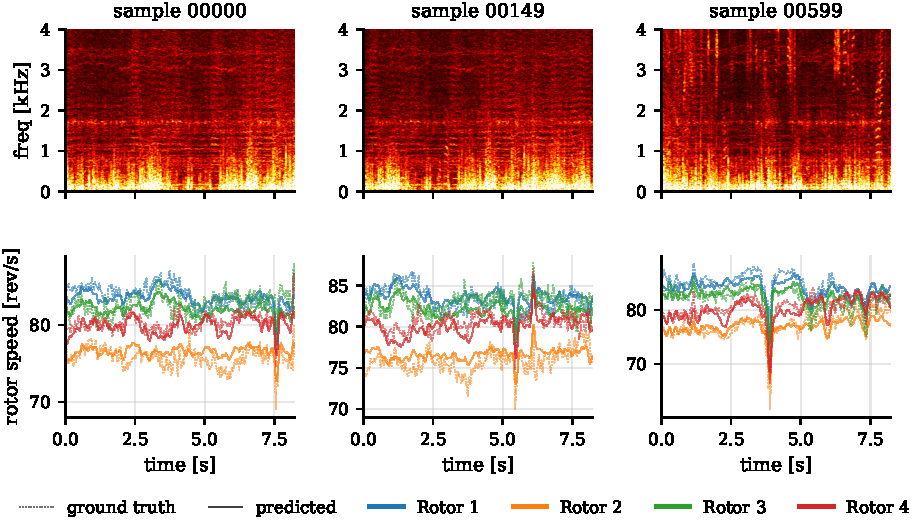
\includegraphics[width=\textwidth]{fig_qualitative_combined}
  \caption{%
    Qualitative SimpleConv predictions on three held-out DREGON-LM validation
    clips.
    \textit{Top}: log-magnitude spectrogram of the mixture (rotor harmonics
    visible as horizontal bands below \SI{2}{\kilo\hertz}; speech occupies
    the upper part of the spectrum).
    \textit{Bottom}: ground-truth (solid) and predicted (dashed) rotor speeds
    for each of the four rotors.
    The four rotors operate at distinct, time-varying speeds; the model tracks
    them individually.%
  }
  \label{fig:qualitative}
\end{figure}

Fig.~\ref{fig:training} shows the training dynamics of SimpleConv.
Validation MSE drops by roughly two orders of magnitude in the first ten epochs
and then settles into a slow refinement phase; the best validation $\rsq$
($0.949$) is reached at epoch~$73$.
Fig.~\ref{fig:qualitative} shows qualitative predictions on three randomly
selected validation clips.
The four rotors operate at clearly distinct speeds, and the predictions track
each rotor individually rather than collapsing onto a single average value.
Most of the residual error consists of fast, low-amplitude fluctuations on top
of an otherwise correct trajectory.

\begin{figure}[ht]
  \centering
  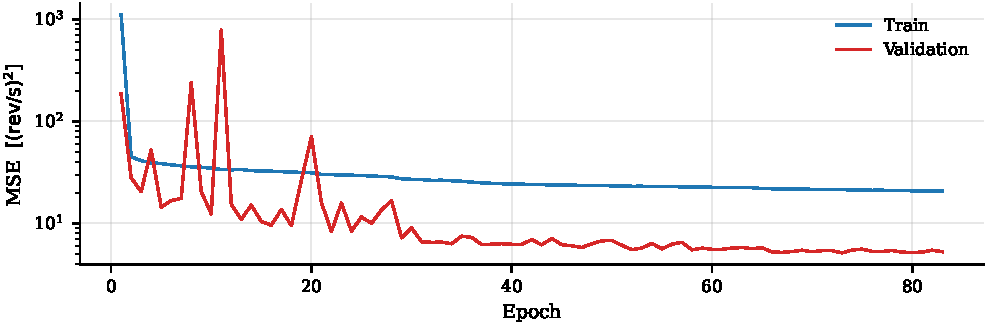
\includegraphics[width=\columnwidth]{fig_training_curves}
  \caption{%
    SimpleConv training dynamics on DREGON-LM.
    (a)~Training and validation MSE on a log scale.
    (b)~Validation $\rsq$.
    The best validation epoch is annotated.%
  }
  \label{fig:training}
\end{figure}

\subsection{Generalisation to real high-SNR free-flight recordings}
\label{sec:highsnr}

The synthetic SNR range $[-30, 0]$~dB is harder than what a typical drone
microphone sees at close range; we therefore additionally evaluate on
out-of-distribution clips taken directly from the DREGON
\emph{free-flight speech-high room1} recording, where a speech source is played
alongside the drone but the speech energy comes from a separate speaker and the
SNR at the on-board microphone is correspondingly higher than in our synthetic
set.
We extract ten non-overlapping $8.22$-second clips evenly spaced through the
recording, run the same three models on the audio without re-training, and
compute per-clip MSE against the synchronised motor telemetry.
Input audio is peak-normalised to $0.9$, matching the normalisation under which
the subset numbers in Table~\ref{tab:main} were obtained.

Fig.~\ref{fig:highsnr} shows the per-clip MSE for each model.
For nine of the ten clips SimpleConv stays close to its in-distribution
performance: the mean MSE across those nine clips is $7.9~(\revps)^{2}$, a
factor of about $1.2$ above its level-matched in-distribution MSE of
$6.84~(\revps)^{2}$.
The complex-valued encoders, which were the stronger models on the
in-distribution subset, degrade much more sharply: mean MSE rises from $3.10$
to $16.4~(\revps)^{2}$ for DCUNet-enc ($\times 5.3$) and from $2.63$ to
$10.0~(\revps)^{2}$ for DCCRN-enc ($\times 3.8$).
The simplest model is by some margin the most robust to the distribution shift
between synthetic mixtures and a real free-flight recording, while the
higher-capacity encoders appear to have fitted features that do not survive
that shift.

The tenth clip (rightmost, around $t \approx 38.6$~s) is an outlier for all
three models.
Inspecting the audio and telemetry, this clip corresponds to a flight phase in
which the drone briefly lands: all four rotor speeds drop to zero, while the
acoustic signature does not change shape correspondingly because residual sounds
(motor wind-down, contact noise) remain.
No model has seen this regime in training---DREGON-LM was constructed from
sustained in-flight noise---so the failure mode is one of distribution shift
rather than of audio-only RPS estimation per se.

\begin{figure}[ht]
  \centering
  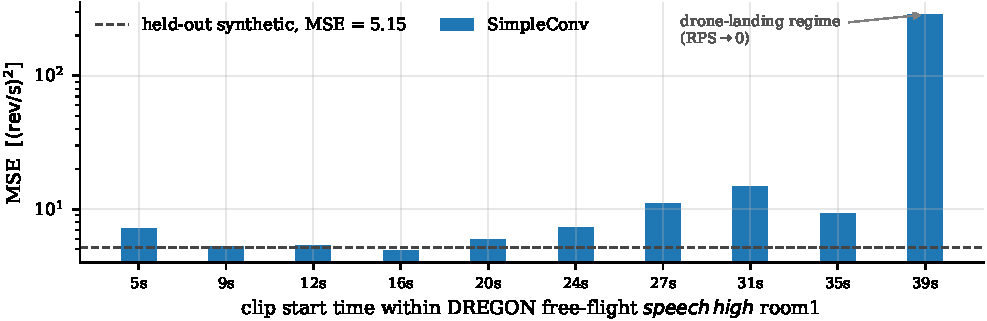
\includegraphics[width=\columnwidth]{fig_highsnr_per_sample}
  \caption{%
    Per-clip MSE on ten consecutive $8.22$-second windows of the DREGON
    \emph{speech-high room1} free-flight recording (out-of-distribution at
    test time).  Dashed line: SimpleConv held-out synthetic-mixture MSE
    ($5.15~(\revps)^{2}$).  The right-most clip corresponds to a brief landing
    phase in which all rotor speeds drop to zero---a regime not represented in
    DREGON-LM training data.%
  }
  \label{fig:highsnr}
\end{figure}

% ============================================================================
\section{Discussion}
% ============================================================================

\textbf{Why is the lightweight model more robust?}
The harmonic comb of a multirotor in flight is a low-dimensional, slowly-varying
object on the magnitude spectrogram: each rotor contributes a small number of
approximately parallel ridges in the time--frequency plane, and the per-rotor
speed determines the spacing of those ridges almost completely.
A small convolutional encoder operating on the log-magnitude STFT already has
the receptive field and inductive bias needed to read this spacing off.
Larger complex-valued encoders, which fit the synthetic mixture distribution
better at training time, appear to do so partly by latching onto features of that
distribution that do not transfer to real free-flight audio.
The robustness result is consistent with the standard reading of
capacity-vs-generalisation trade-offs on small datasets, with the additional
twist that here the in-distribution \emph{ranking} of architectures reverses out
of distribution; we view this as a useful caution against over-interpreting
in-distribution rankings on small drone-acoustics datasets in general.

\textbf{Limitations.}
Three limitations bound the conclusions.
First, both training and evaluation use a single quadcopter platform (the DREGON
drone); generalisation across airframes, propellers and microphone configurations
is untested and is the natural next experiment.
Second, the held-out synthetic set shares underlying drone recordings with the
training set (different clips, same flights), so part of $\rsq$ reflects
in-distribution interpolation; the high-SNR free-flight analysis is the strongest
evidence against this but remains small.
Third, ground-truth speeds are interpolated from a motor-sampled tachometer onto
the STFT time grid, so fast transients are smoothed and we do not currently
report errors as a function of $\dot{\mathbf{r}}(t)$.

\textbf{Outlook.}
The result is a feasibility study: audio-only multi-rotor RPS estimation is
tractable, with a small model, at SNRs that include speech-dominated mixtures.
Two follow-ups are obvious:
(i) careful comparison against classical baselines---single-$f_{0}$ trackers,
cepstral analysis, harmonic-product spectra, and matched-filter banks indexed
by RPS---to quantify what the learned model buys over signal processing,
especially in the hardest regime; and
(ii) use of the predicted RPS as a conditioning signal for downstream tasks,
whose tolerance to RPS error needs to be measured rather than assumed.

% ============================================================================
\section{Conclusion}
% ============================================================================

We have presented a first study of audio-only rotor speed estimation for
multirotor UAVs in the presence of strong non-rotor sound.
A small convolutional regressor trained on synthetic LibriSpeech--DREGON mixtures
predicts per-rotor speed across an SNR range of $-30$ to $0$~dB with
$\rsq = 0.95$ and a mean absolute error of $0.56~\revps$, and remains accurate
on real high-SNR free-flight recordings except in flight regimes (landing) not
represented in the training distribution.
The result establishes that the dominant acoustic structure of a multirotor in
flight carries enough information about its rotational state to make passive
acoustic monitoring of drone state feasible without onboard telemetry, and
motivates a more systematic study of audio-only drone-state estimation as a
useful primitive in its own right.

%%%%%%%%%%%%%%%%%%%%%%%%%%%%%%%%%%%%
% ACKNOWLEDGEMENTS
%%%%%%%%%%%%%%%%%%%%%%%%%%%%%%%%%%%%
\section*{Acknowledgments}
% TODO: add funding acknowledgements
%%%%%%%%%%%%%%%%%%%%%%%%%%%%%%%%%%%%
% END OF ACKNOWLEDGEMENTS
%%%%%%%%%%%%%%%%%%%%%%%%%%%%%%%%%%%%

%%%%%%%%%%%%%%%%%%%%%%%%%%%%%%%%%%%%
% REFERENCES
%%%%%%%%%%%%%%%%%%%%%%%%%%%%%%%%%%%%
\bibliography{refs}
\bibliographystyle{apacite}
%%%%%%%%%%%%%%%%%%%%%%%%%%%%%%%%%%%%
% END OF REFERENCES
%%%%%%%%%%%%%%%%%%%%%%%%%%%%%%%%%%%%

\end{document}
